
%%%%%%%%%%%%%%%%%%%%%%%%%%%%%%%%%%%%%%%%%%%%%%%%%%%%%%%%%%%%%%%%%%%%%
%% This is a (brief) model paper using the achemso class
%% The document class accepts keyval options, which should include
%% the target journal and optionally the manuscript type.
%%%%%%%%%%%%%%%%%%%%%%%%%%%%%%%%%%%%%%%%%%%%%%%%%%%%%%%%%%%%%%%%%%%%%
\documentclass[journal=jctcce,manuscript=article]{achemso}

%%%%%%%%%%%%%%%%%%%%%%%%%%%%%%%%%%%%%%%%%%%%%%%%%%%%%%%%%%%%%%%%%%%%%
%% Place any additional packages needed here.  Only include packages
%% which are essential, to avoid problems later. Do NOT use any
%% packages which require e-TeX (for example etoolbox): the e-TeX
%% extensions are not currently available on the ACS conversion
%% servers.
%%%%%%%%%%%%%%%%%%%%%%%%%%%%%%%%%%%%%%%%%%%%%%%%%%%%%%%%%%%%%%%%%%%%%
\usepackage[version=3]{mhchem} % Formula subscripts using \ce{}
\usepackage[T1]{fontenc}       % Use modern font encodings
\usepackage{amsmath}	    % American Mathematical Society equation formatting
\graphicspath{ {images/} }     % Path to images
%TO REMOVE BEFORE SUBMISSION
\usepackage{lineno} % add the line numbers
\linenumbers
%END TO REMOVE BEFORE SUBMISSION

%%%%%%%%%%%%%%%%%%%%%%%%%%%%%%%%%%%%%%%%%%%%%%%%%%%%%%%%%%%%%%%%%%%%%
%% If issues arise when submitting your manuscript, you may want to
%% un-comment the next line.  This provides information on the
%% version of every file you have used.
%%%%%%%%%%%%%%%%%%%%%%%%%%%%%%%%%%%%%%%%%%%%%%%%%%%%%%%%%%%%%%%%%%%%%
%%\listfiles

%%%%%%%%%%%%%%%%%%%%%%%%%%%%%%%%%%%%%%%%%%%%%%%%%%%%%%%%%%%%%%%%%%%%%
%% Place any additional macros here.  Please use \newcommand* where
%% possible, and avoid layout-changing macros (which are not used
%% when typesetting).
%%%%%%%%%%%%%%%%%%%%%%%%%%%%%%%%%%%%%%%%%%%%%%%%%%%%%%%%%%%%%%%%%%%%%
\newcommand*\mycommand[1]{\texttt{\emph{#1}}}

%%%%%%%%%%%%%%%%%%%%%%%%%%%%%%%%%%%%%%%%%%%%%%%%%%%%%%%%%%%%%%%%%%%%%
%% Meta-data block
%% ---------------
%% Each author should be given as a separate \author command.
%%
%% Corresponding authors should have an e-mail given after the author
%% name as an \email command. Phone and fax numbers can be given
%% using \phone and \fax, respectively; this information is optional.
%%
%% The affiliation of authors is given after the authors; each
%% \affiliation command applies to all preceding authors not already
%% assigned an affiliation.
%%
%% The affiliation takes an option argument for the short name.  This
%% will typically be something like "University of Somewhere".
%%
%% The \altaffiliation macro should be used for new address, etc.
%% On the other hand, \alsoaffiliation is used on a per author basis
%% when authors are associated with multiple institutions.
%%%%%%%%%%%%%%%%%%%%%%%%%%%%%%%%%%%%%%%%%%%%%%%%%%%%%%%%%%%%%%%%%%%%%
\author{Alexander Punter}
\author{Paola Nava}
\author{Yannick Carissan}
\email{Yannick.Carissan@univ-amu.fr}
\phone{+33 (0)491289168}
\affiliation[Aix-Marseille University]
{Aix Marseille Univ, CNRS, Centrale Marseille, iSm2, Marseille, France}
%%%%%%%%%%%%%%%%%%%%%%%%%%%%%%%%%%%%%%%%%%%%%%%%%%%%%%%%%%%%%%%%%%%%%
%% The document title should be given as usual. Some journals require
%% a running title from the author: this should be supplied as an
%% optional argument to \title.
%%%%%%%%%%%%%%%%%%%%%%%%%%%%%%%%%%%%%%%%%%%%%%%%%%%%%%%%%%%%%%%%%%%%%
\title[A great title]
  {A great title}

%%%%%%%%%%%%%%%%%%%%%%%%%%%%%%%%%%%%%%%%%%%%%%%%%%%%%%%%%%%%%%%%%%%%%
%% Some journals require a list of abbreviations or keywords to be
%% supplied. These should be set up here, and will be printed after
%% the title and author information, if needed.
%%%%%%%%%%%%%%%%%%%%%%%%%%%%%%%%%%%%%%%%%%%%%%%%%%%%%%%%%%%%%%%%%%%%%
\abbreviations{IR,NMR,UV}
\keywords{Pseudo potentials, Group potentials}

%%%%%%%%%%%%%%%%%%%%%%%%%%%%%%%%%%%%%%%%%%%%%%%%%%%%%%%%%%%%%%%%%%%%%
%% The manuscript does not need to include \maketitle, which is
%% executed automatically.
%%%%%%%%%%%%%%%%%%%%%%%%%%%%%%%%%%%%%%%%%%%%%%%%%%%%%%%%%%%%%%%%%%%%%
\begin{document}

%%%%%%%%%%%%%%%%%%%%%%%%%%%%%%%%%%%%%%%%%%%%%%%%%%%%%%%%%%%%%%%%%%%%%
%% The "tocentry" environment can be used to create an entry for the
%% graphical table of contents. It is given here as some journals
%% require that it is printed as part of the abstract page. It will
%% be automatically moved as appropriate.
%%%%%%%%%%%%%%%%%%%%%%%%%%%%%%%%%%%%%%%%%%%%%%%%%%%%%%%%%%%%%%%%%%%%%
\begin{tocentry}

Some journals require a graphical entry for the Table of Contents.
This should be laid out ``print ready'' so that the sizing of the
text is correct.

Inside the \texttt{tocentry} environment, the font used is Helvetica
8\,pt, as required by \emph{Journal of the American Chemical
Society}.

The surrounding frame is 9\,cm by 3.5\,cm, which is the maximum
permitted for  \emph{Journal of the American Chemical Society}
graphical table of content entries. The box will not resize if the
content is too big: instead it will overflow the edge of the box.

This box and the associated title will always be printed on a
separate page at the end of the document.

\end{tocentry}

%%%%%%%%%%%%%%%%%%%%%%%%%%%%%%%%%%%%%%%%%%%%%%%%%%%%%%%%%%%%%%%%%%%%%
%% The abstract environment will automatically gobble the contents
%% if an abstract is not used by the target journal.
%%%%%%%%%%%%%%%%%%%%%%%%%%%%%%%%%%%%%%%%%%%%%%%%%%%%%%%%%%%%%%%%%%%%%
\begin{abstract}
A pseudo-potential system for recreating an sp\(^{2}\) carbon atom is built 
and tested as a building block for various pseudo-hydrocarbon chain and ring systems.  
This pseudo-system has a central charge of 1, thus it contains only one
electron. It has been employed in \textsl{ab-initio} calculations:
1\textsuperscript{st} ionisation and excitation energies, as well as the HOMO energy, 
are found to be reproduced to a good accuracy by the pseudo-system.
\end{abstract}

%%%%%%%%%%%%%%%%%%%%%%%%%%%%%%%%%%%%%%%%%%%%%%%%%%%%%%%%%%%%%%%%%%%%%
%% Start the main part of the manuscript here.
%%%%%%%%%%%%%%%%%%%%%%%%%%%%%%%%%%%%%%%%%%%%%%%%%%%%%%%%%%%%%%%%%%%%%
\section{Introduction}

\newcounter{customItem}
\newcommand{\showCustomItem}{\refstepcounter{customItem}\roman{customItem}}

%For most of the quantum chemistry calculations, the system can be divided into two parts:
%the active part, \emph{i.e.} the part of the molecule one is interested in and
%the inactive part, which is to be taken into account in order to fulfill chemical requirements.
It is a common idea that a chemical system can be thought as constituted by (at least) 
two parts:
an active one, where most of the chemistry takes place, and an (apparently) inactive
one, which must be taken into account in order to fulfill chemical requirements.
Based on this general statement, many successful theoretical approaches were developped.
Among them,  QM/QM' or QM/MM methods (\showCustomItem) can be cited, where 
the active region that usually contains several atoms, is
treated at a high level of calculation, while the inactive part is treated at a 
lower level of theory.\cite{chung_oniom_2015}
Frozen density embedding techniques (\showCustomItem) replace part of a molecule or 
its surrounding
by a frozen electronic density extracted on a reference system.\cite{wesolowski_frozen-density_2015}
They are an extension of the frozen core approximation, already used %in the early days 
to reduce
the number of parameters to be optimized in the self consistent field calculation.REF?

In this article we shall focus on pseudo-potential techniques, which also
divide the chemical problem into two parts.
Effective core potentials (\showCustomItem) are commonly employed for atoms: 
core electrons are
replaced by an operator fast to evaluate and the active electrons are treated
explicitly.\cite{dolg_relativistic_2012}
In the same vein, model potentials (\showCustomItem) replace a frozen electronic density (computed on the atom)
by some operators, the number of which depends on the level of
refinement required.\cite{huzinaga_1994_1995}

The effective group potentials (\showCustomItem) bridge the frozen density and the core potential
approaches: using core potential extraction techniques, effects due to the implicit 
electron density are reproduced by a mono-electronic operator.\cite{carissan_what_2006}
However, while effective core potentials and model potentials intend to 
reproduce atomic properties,
effective group potentials aim at mimicking the effect of atoms involved in one or more chemical
bonds. The cyclopentadienyl group was, for instance, successfully extracted.
In this example, carbon atoms are hybridized and the core/valence distinction is not 
strictly defined.
Let us follow Huzinaga in his enlightening work.\cite{huzinaga_effective_1991}
In order to extract a meaningful potential, he states that for electron/electron interactions, 
"the most important effect is that the exclusion principle prevents active electrons
from collapsing into the dormant region.
The second is the exchange energy terms between the dormant and active electrons
through their electrostatic interaction."
For an atom, the Hamiltonian reads:
\begin{equation}
\label{eq:atomicHamiltonian}
\hat{H} = \sum_{i=1}^n \hat{h}(i) +\sum_{i<j}\frac{1}{r_{ij}}
\end{equation}
with $\frac{1}{r_{ij}}$ the bielectronic interaction
between explicitly treated active electrons and
the mono electronic operator:
\begin{equation}
\label{eq:monoElectronicOperator}
\hat{h}(i) = -\frac{1}{2}\Delta_i - \frac{(Z-Z_c)}{r_i}+\hat{V}(i) + \hat{\sigma}(i)
\end{equation}
where
$\Delta_i$ is the laplacian of the coordinates of electron $i$,
$Z_C$ is the number of core electrons withdrawn from the reference system,
$\hat{V}(i)$ the pseudo potential which reproduces the electrostatic
interaction between the dormant and active electrons
and $\hat{\sigma}(i)$ the operator, which models the exclusion principle
and prevents active electrons from collapsing into the dormant region.
To take into account the fact that dormant electrons are removed from the
system, the nuclear charge is modified by the $Z_c$ value.
Yet, as the effective charge felt by the active electrons is likely not to be an integer,
the modification of the value of the nuclear charge is scaled in $\hat{V}$.
Depending on the version used, this modification differs.
In this work, we take as a reference version 1 as defined in
Huzinaga's lecture\cite{huzinaga_1994_1995}:
\begin{equation}
\label{eq:HuzinagaMPVersion1Potential}
\hat{V} = \frac{1}{r}\left[\sum_IA_I\exp(-\alpha r^2)+\sum_JB_Jr\exp(-\beta r^2)\right]
\end{equation}
In this model potential version, $\hat{\sigma}$ is defined as:
\begin{equation}
\label{eq:HuzinagaMPVersion1Sigma}
\hat{\sigma} = -\sum f_c\epsilon_c\left|\phi_c\right>\left<\phi_c\right|
\end{equation}
with $\epsilon_c$ the eigenvalue of the core orbital $\phi_c$ and
$f_c$ an optimized parameter.
In the other versions of model potentials, $f_c=2$, as suggested earlier.\cite{houjer_aspects_1978}
In the present work, we shall optimize the parameters in $\hat{V}$ and $\hat{\sigma}$
for hybridized atoms.
Before going further, it is important to stress that hybridization implies that the
$\left\{\phi_c\right\}_i$ are linear combination of atomic orbitals and that
$\hat{V}$ should no more be spherical.
This loss of isotropy combined with the loss of clear core/valence separation
will imply constraints during the extraction process.

In this work, we aim at developing a method usable out of the box in any standard
quantum chemistry software.
Thus, no modification of the source code should be done.
This supplementary constraint will be fulfilled by strategically positioning the pseudo potentials
we intend to use. 
We have already successfully used this technique to extract pseudo potentials for hybridized carbon
atoms.\cite{drujon_pseudopotentials_2013}
However, in our extraction procedure, some pseudo potentials had to be put precisely at the center
of each bond.
Thus, those pseudo potentials could not be considered as atomic as they were not only defined
with respect to the position of the atom they applied to.
In this new version, the pseudo potentials are fully atomic: the position of the atom
determines completely where the potentials are put in space in the best possible manner
when dealing with hybridized atoms (as hybridization destroys anisotropy, the preferred orientations
must be given to define the pseudo potential).

This article is structured as follows.
In the first part, the method is defined in detail.
The second part shows the results obtained, from the most crude to the most refined
version of the method.
These are analyzed in the third part.

\section{Method}

\subsection{Potentials \& Potential Geometry}

As in our previous work\cite{drujon_pseudopotentials_2013},
we take a CH\(^{\bullet}_{3}\) as our starting system to be reproduced.
It is the smallest system containing one and only one sp$^2$ hybridized carbon atom.
This choice allows us to isolate the different electrostatic interactions
to build a physically meaningful model.
In order to fulfil the criteria specified in Equation (\ref{eq:atomicHamiltonian}),
we make use of two kinds of Gaussian pseudo-potentials \cite{me_structure_theory}, of \(s\) and \(p\) shapes. As we want to avoid modifying the quantum chemistry software itself, the pseudo-potentials have a semi-local form and we choose a value of \(n = 1\) to preserve the \(1/r\) behaviour as in Huzinanaga's work. As will be discussed in the following sections,
the \(p\) pseudo-potential allows to reproduce atomic properties, when the
\(s\)-potentials mimic electrostatic electron pair repulsion. The pseudo-potentials are monoelectronic operators, thus they shall not be able to reproduce fully bielectronic interactions. Knowing this, we adjust the parameters of the \(s\)-potentials for the pseudo-system to have a wavefunction in which properties are as close as possible to those of the reference system, such as spatial extent, energy and excitation energies.

\begin{figure}[ht]
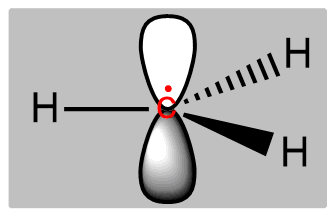
\includegraphics[width=8cm]{ch3.png}
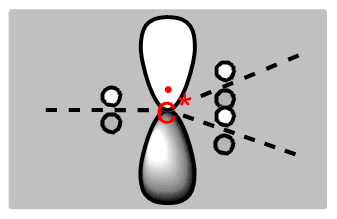
\includegraphics[width=8cm]{pseudoch3.png}
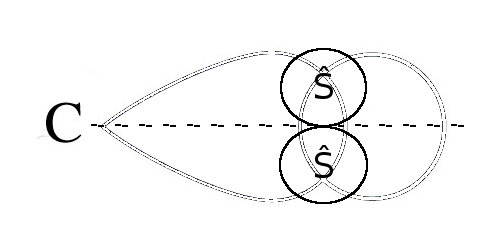
\includegraphics[width=8cm]{tm_sp2_potentials.png}
\caption{Diagrams of CH\(^{\bullet}_{3}\) (left) and pseudo-CH\(^{\bullet}_{3}\) (right, below) molecules. The pseudo-CH\(^{\bullet}_{3}\) diagrams display the \(s\) and \(p\)-potential positions, and the distances \(d\) and \(c\).}
\label{figure:ref_pseudo_diagram}
\end{figure}

Figure \ref{figure:ref_pseudo_diagram} displays the final pseudo-system: The CH\(^{\bullet}_{3}\) radical has been replaced by
a hydrogen-like "pseudo-carbon", with a nuclear charge of \(Z_{nucleus} = 1\), and one electron occupying the \(p_{z}\) orbital. 
There are now no H atoms, and the system is surrounded by three potential sets at a planar distance of \(d\), each consisting of 
two \(s\)-shaped potentials with a distance above and below the \(xy\)-plane of \(c\). A further \(p\)-shaped potential is applied
directly to the pseudo-carbon.

This gives multiple variables we can use to manipulate the properties of the system.
We can alter the strength and diffuseness of the \(p\) and \(s\) potentials themselves,
as well as vary the distances \(d\) and \(c\) by moving the \(s\)-potentials.
In this article, we fix \(c = 0.25\;a.u.\).

\subsection{Making Potentials Physically Meaningful}
\label{section:potential_derivation}

It is possible to obtain the potential parameters entirely by empirical means. However, we can make a more informed guess at some starting parameters from which to optimise. Clearly the assumption that \(Z = 1\) is unrealistic. Slater's Rules\cite{slatersrules} suggest that, with the screening effect, the \(p_{z}\) electron of a carbon atom should experience a charge of \(Z = 2.4\). To mimic the effect of an electron-screened nucleus, we can use a \(p_{z}\) pseudo-potential. In order to make an educated guess of the parameters of this new potential, we need to find an expression for \(Z_{eff}(\langle r \rangle)\); \(Z_{eff}\) being the total nuclear attraction the electron would feel in the real CH\(^{\bullet}_{3}\) system, taking into account the screening effect of the core electrons that would be present in an all-electron model; and \( \langle r \rangle \) being the expected distance of the electron from the nucleus.
%%	The generic forms of Gaussian Type Orbitals for \(s\) and \(p_{z}\) are [REF]
%% \begin{equation}
%% \psi_{s} = re^{-\alpha r^{2}},\qquad	\psi_{p_{z}} = r \cos \theta e^{-\alpha r^{2}}
%% \end{equation}

The analytical form of the \(p_{z}\) orbital for a hydrogen-like atom is\cite{nyu_h_solutions}
\begin{equation}
\phi_{210} = \frac{1}{\sqrt{\pi}} \frac{Z_{eff}}{2a_{0}} ^{\frac{5}{2}} re^{-\frac{Z_{eff}r}{2a_{0}}} \cos \theta
\end{equation}
and from this we obtain 
\begin{equation}
\label{equation:PsirPsi}
\langle \phi_{210} | r | \phi_{210} \rangle = \frac{5a_{0}}{Z_{eff}}
\end{equation}
Next, we need to find a value for \( \langle r \rangle \). We can do this by calculating
\begin{equation}
\langle r \rangle = \lambda B \lambda^{T}
\label{equation:exp_r}
\end{equation}
where \(\lambda\) are the Symmetrised Atomic Orbital Shells taken from the molecular orbital files of a reference Turbomole calculation of a CH\(^{\bullet}_{3}\) radical, and B is the matrix of \(\langle \psi_{p_{z}} | r | \psi_{p_{z}} \rangle\) values, appropriately normalised and contracted according to the basis set used (in this case, def-SV(P) \cite{defsvp}).

From Equation \ref{equation:exp_r}, we have \( \langle r \rangle \approx 1.8\;a.u.\) and therefore we can see from Equation \ref{equation:PsirPsi} that \(Z_{eff} \approx 3.6\). Even if we shall use the semi-local pseudopotential definition for the calculations, for a quick evaluation of overlap effects between the basis set and the pseud-opotential, we assume a non-local pseudo-potential definition. We define:
\begin{equation}
S = \langle \phi_{p_{z}} | \chi \rangle
\end{equation}
the overlap between a molecular orbital \(\phi_{p_{z}}\), and \(\chi\), taken from our non-local pseudo-potential definition \cite{huzinaga_effective_1991}
\begin{equation}
\chi = e^{-\alpha r^{2}},\qquad \widehat{p} = Z_{pseudo} | \chi \rangle \langle \chi |
\end{equation}
leading us to
\begin{equation}
\langle \widehat{Z} \rangle = \langle \phi_{p_{z}} | \widehat{Z} | \phi_{p_{z}} \rangle = \langle \phi_{p_{z}} | Z_{pseudo} | \chi \rangle \langle \chi | \phi_{p_{z}} \rangle = Z_{pseudo} S^{2}
\end{equation}
Finally, knowing that our hydrogen-like pseudo-system already contains a charge, \(Z_{nucleus}\), of one we subtract this from the desired \(Z_{eff}\) we want to influence our \(p_{z}\) electron, leaving us with
\begin{equation}
Z_{pseudo} = (Z_{eff} - Z_{nucleus})S^{-2}
\end{equation}

We now have the power to choose a \(p_{z}\) pseudo-potential solely based on the Gaussian exponent, and the \(Z_{eff}\) then follows from the above. Clearly, the exponent should be chosen to give us a strong overlap. Hence we arrive at a \(p_{z}\)-potential that should be physically meaningful. 

\subsection{Computational Details}

Here summarised are details of the methods used in calculation. All Hartree-Fock, DFT and time-dependent DFT (TD-DFT) energy calculations are performed with TURBOMOLE 7.1 \cite{TURBOMOLE}. The basis set used throughout is def-SV(P) \cite{defsvp}. Wherever possible, planar (C\(_{S}\)) symmetry is used. The convergence energy is \(10^{-7}\)H (\texttt{\$scfconv = 7}) for SCF and \(10^{-6}\)H for DFT. When running these calculations the occupation of orbitals is specified manually in the TURBOMOLE control file.

\textbf{Chain Alkenes, Ring Molecules}. In additional to Hartree-Fock calculations, DFT is used with PBE0, PBE, TPSS and TPSSh functionals. \cite{pbe0,pbe,tpss,tpssh} The integration grid size is set at \(m4\). Also used are TD-DFT calculations, where the Tamm-Dancoff approximation (CIS) \cite{tammdancoff} is switched on to avoid triplet instability.

\section{Results, Development and Discussion}
\subsection{CH\(_{3}\), with \(s\)-potentials}

%\begin{table}[ht]
%\caption{Reference values and \(s\)-only pseudo-system values for CH\(^{\bullet}_{3}\), optimised to give the correct HOMO energy. \(d = 0.5\) a.u.}
%\begin{tabular}{c c c}
%\hline
%\multicolumn{3}{c}{Reference} \\
%\hline\hline
%Calculation Type & \multicolumn{2}{c}{CH\(^{\bullet}_{3}\)\, HOMO (\(p_{z}\)) energy (eV)} \\
%\hline
%HF & \multicolumn{2}{c}{-10.537} \\
%PBE0 & \multicolumn{2}{c}{-6.726} \\
%\hline
%\multicolumn{3}{c}{Pseudo-system} \\
%\hline\hline
% & Coefficient & Exponent \\ [0.5ex]
%\hline
%HF & -2.594 & 1.0 \\
% & -4.788 & 5.0 \\
% & -7.524 & 10.0 \\
%\hline
%PBE0 & -2.605 & 1.0 \\
% & -4.873 & 5.0 \\
% & -7.678 & 10.0 \\
%\hline
%\end{tabular}
%\label{table:ch3_s_potentials}
%\end{table}

\begin{table}[ht]
\caption{Coefficients and exponents for \(s\)-only pseudo-potentials for CH\(^{\bullet}_{3}\), optimised to give 
the all-electron HOMO reference energy of  -10.537~eV (HF) and -6.726~eV (PBE0). 
\(d = 0.5\) a.u., as defined in Figure~\ref{figure:ref_pseudo_diagram}.}
\begin{tabular}{c c c}
\hline
%\multicolumn{3}{c}{Reference} \\
%\hline\hline
%Calculation Type & \multicolumn{2}{c}{CH\(^{\bullet}_{3}\)\, HOMO (\(p_{z}\)) energy (eV)} \\
%\hline
%HF & \multicolumn{2}{c}{-10.537} \\
%PBE0 & \multicolumn{2}{c}{-6.726} \\
%\hline
%\multicolumn{3}{c}{Pseudo-system} \\
%\hline\hline
 & Coefficient & Exponent \\ [0.5ex]
\hline
HF & -2.594 & 1.0 \\
 & -4.788 & 5.0 \\
 & -7.524 & 10.0 \\
\hline
PBE0 & -2.605 & 1.0 \\
 & -4.873 & 5.0 \\
 & -7.678 & 10.0 \\
\hline
\end{tabular}
\label{table:ch3_s_potentials}
\end{table}

\begin{figure}
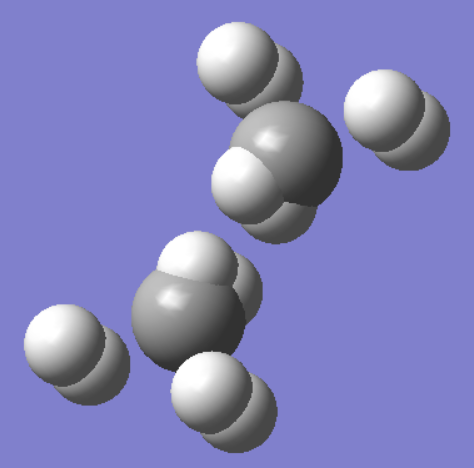
\includegraphics[width=8cm]{long_r_ethene_diagram.png}
\caption{Diagram of pseudo-ethene displaying pseudo-carbon atoms (grey) and \(s\) pseudo-potentials (white).}
\label{fig:long_r_ethene}
\end{figure}

We aim first at reproducing the values for the CH\(^{\bullet}_{3}\) radical as given in Table \ref{table:ch3_s_potentials}. This reference CH\(^{\bullet}_{3}\) is created and has its geometry optimised under Hartree-Fock. The pseudo-system is then set up, erasing the hydrogen atoms, setting the carbon charge \(Z_{nucleus} = 1\) and applying \(s\) pseudo-potentials, as well as selecting the correct orbital for the remaining electron. Table \ref{table:ch3_s_potentials} displays some of our results. Promisingly, we are able to produce many sets of potentials that give the correct energy with coefficients and exponents of the same order of magnitude as the basis set.

\subsection{Ethene, with \(s\) and \(p\)-potentials}

Next, we take some of these potentials to create a pseudo-ethene system, with the results shown in Table \ref{table:ethene_s_pseudo}. All potentials tested with \(d = 2.0\) a.u. gave results several orders of magnitude away from the reference value. From Figure \ref{fig:long_r_ethene} we may see the reason. One of the potential sets from each carbon is closer to the neighbouring carbon than the neighbour's own potential sets, thus both pseudo-carbons are affected by potentials which do not belong to them. At the shorter range \(d = 0.5\) a.u., the HOMO energy is of the right magnitude, though with errors of \(~ 30\%\). Attempts to eliminate this error lead us to the additional use of the \(p_{z}\) potential \textit{alongside} the \(s\) potentials.

%\begin{table}[ht]
%\caption{Reference values and HOMO-optimised values for Pseudo-ethene using only \(s\)-potentials with an exponent of 10.0}
%\begin{tabular}{c c c}
%\hline
%\multicolumn{3}{c}{Reference} \\
%\hline\hline
%Calculation Type & \multicolumn{2}{c}{C\(_{2}\)H\(_{4}\)\ HOMO )\(\pi\)) energy (eV)} \\
%\hline
%HF & \multicolumn{2}{c}{-10.363} \\
%PBE0 & \multicolumn{2}{c}{-6.632} \\
%\hline
%\multicolumn{3}{c}{Pseudo-system} \\
%\hline\hline
% & \(s\) coefficient & \( \pi \) orbital energy (eV) \\
%\hline
%\multicolumn{3}{c}{d = 2.0 a.u.} \\
%\hline
%HF & -7.521 & -9597.0 \\
%\hline
%\multicolumn{3}{c}{d = 0.5 a.u.} \\
%\hline
%HF & -7.521 & -7.905 \\
%PBE0 & -7.679 & -8.447 \\
%\hline
%\end{tabular}
%\label{table:ethene_s_pseudo}
%\end{table}

\begin{table}[ht]
\caption{Reference values and HOMO-optimised values for Pseudo-ethene using only \(s\)-potentials with an exponent of 10.0.
$d$ (a.u.) as defined in Figure~\ref{figure:ref_pseudo_diagram}.}
\begin{tabular}{c c c c}
\hline
%\multicolumn{3}{c}{Reference} \\
%\hline\hline
%Calculation Type & \multicolumn{2}{c}{C\(_{2}\)H\(_{4}\)\ HOMO )\(\pi\)) energy (eV)} \\
%\hline
%HF & \multicolumn{2}{c}{-10.363} \\
%PBE0 & \multicolumn{2}{c}{-6.632} \\
%\hline
%\multicolumn{3}{c}{Pseudo-system} \\
%\hline\hline
& $d$ & \(s\) coefficient & \( \pi \) orbital energy (eV) \\
\hline
HF$^a$   &     &        & -10.363 \\
PBE0$^a$ &     &        & -6.632 \\
HF       & 2.0 & -7.521 & -9597.0 \\
HF       & 0.5 & 7.521  & -7.905 \\
PBE0     & 0.5 &-7.679  & -8.447 \\
\hline
\multicolumn{4}{l}{$^a$ All-electron reference values.}\\
\end{tabular}
\label{table:ethene_s_pseudo}
\end{table}

The next step adds a \(p\)-potential centred on the pseudo-carbon, with Table \ref{table:p_potentials} displaying the results. As before, \(d = 0.5\) a.u.. The \(p_{z}\) potential is selected using the procedure described in Section \ref{section:potential_derivation}, with the exponent chosen to give the maximum possible overlap with the \(p_{z}\) orbital, and the matching \(Z_{eff}\) coefficient calculated from the exponent and overlap. The \(s\)-potentials are then optimised once more to give the correct HOMO energy for CH\(^{\bullet}_{3}\). We again take these potentials to create a pseudo-ethene molecule, with the results shown in Table \ref{table:p_potentials}. We can see that these potentials seem to transfer more effectively from the CH\(^{\bullet}_{3}\) system to the ethene, suggesting therefore that whilst the \(s\)-potentials can affect both the \(p_{z}\) and \(\pi\) orbitals, they cannot alone represent the relationship between them.

Having successfully created a pseudo-ethene with the correct HOMO, we attempt to have the pseudo-system replicate other properties of the real system. Reference values for the singlet-triplet \(\pi-\pi*\) excitation and first ionisation energies of ethene are given in Table \ref{table:ethene_excitations}. Testing the relevant energies for the pseudo-systems, the early results are not promising, as we can see from Table \ref{table:ethene_excitations}. However, after we abandon the notion of sticking strictly to a \(p_{z}\)-potential exponent that gives the maximum overlap with the real orbital, we discover there is a "sweet spot" of potential coefficients and exponents around which the correct values begin to emerge. Table \ref{table:ethene_excitations} shows our optimal result, chosen to give HOMO, excitation and ionisation energies closest to the reference values. 

\begin{table}[ht]
\caption{Optimised s-orbital pseudopotentials for pseudo-CH\(^{\bullet}_{3}\) and pseudo-ethene. \(d = 0.5\) a.u.}
\begin{tabular}{c c c c}
\hline
& \(p\) coefficient & \(p\) exponent \\
\hline
\(p_{z}\) potential & -3.267 & 0.295 \\
%\hline
%Calculation Type & \(s\) coefficient & \(s\) exponent &  \\
%\hline
%\multicolumn{3}{c}{CH\(^{\bullet}_{3}\)} \\
%\hline\hline
%HF & 2.772 & 1.0 &  \\
% & 6.173 & 5.0 &  \\
% & 10.381 & 10.0 &  \\
%\hline
%PBE0 & 3.483 & 1.0 &  \\
% & 9.801 & 5.0 &  \\
% & 18.351 & 10.0 &  \\
\hline
%\multicolumn{3}{c}{Ethene} & \(\pi\) orbital energy (eV) \\
Calculation Type & \(s\) coefficient & \(s\) exponent & \(\pi\) \\
\hline\hline
HF & 2.772 & 1.0 & -13.654 \\
 & 6.173 & 5.0 & -14.011 \\
 & 10.381 & 10.0 & -14.061 \\
\hline
PBE0 & 3.483 & 1.0 & -10.325 \\
 & 9.801 & 5.0 & -10.409 \\
 & 18.351 & 10.0 & -12.543 \\
\hline
\end{tabular}
\label{table:p_potentials}
\end{table}

\begin{table}[ht]
\caption{\(s\)-potential fits to ethene \(\pi-\pi*\) excitation}
\begin{tabular}{c c c c c}
\hline
\(s\)-coefficient & \(s\)-exponent & Excitation (eV) & Ionisation (eV) & HOMO energy (eV) \\
\hline
%\multicolumn{5}{c}{Reference System} \\
%\hline\hline
%& & -3.533 & -9.091 & -10.363 \\
%\hline
%\multicolumn{5}{c}{Pseudo-Systems} \\
%\hline\hline
\multicolumn{2}{c}{Reference Values} & -3.533 & -9.091 & -10.363 \\
\hline
\multicolumn{5}{c}{\(p\)-coefficient -3.267; \(p\)-exponent 0.295} \\
\hline
0.552 & 0.1 & -3.533 & -27.158 & -27.31 \\
0.608 & 1.0 & -3.533 & -28.247 & -28.395 \\
0.936 & 5.0 & -3.533 & -29.583 & -29.722 \\
\hline
\multicolumn{5}{c}{\(p\)-coefficient -3.91; \(p\)-exponent 0.624} \\
\hline
1.5 & 0.5 & -3.533 & -9.806 & -10.062 \\
\hline
\end{tabular}
\label{table:ethene_excitations}
\end{table}

\subsection{C\(_{2n}\)H\(_{2n+2}\)}

Taking these new potentials we test them against a series of chain alkenes up to length C\(_{12}\), using a variety of functionals. In each case, the geometry of the reference system is optimised according to the method used, before taking the reference geometry and applying the pseudo-potentials from Table \ref{table:ethene_excitations}, optimised for ethene under HF. Figures \ref{fig:alkenes_hf_dft} and \ref{fig:alkenes_tddft} show the results. Table \ref{table:alkene_errors} gives a breakdown of the percentage errors for each method across all molecules tested. The pattern of increasing HOMO energy and decreasing ionisation and excitation energies seen in the reference systems seems to be well replicated by the pseudo-alkenes, with the energies following the same gradient. [COMMENT on ERRORS]

Also compared are TD-DFT results for this system and that in Carissan and Drujon \cite{drujon_pseudopotentials_2013}, which match to within 3\%. It seems the previous results have been accurately replicated.
Let us remind here that unlike in our previous work\ref{drujon_pseudopotentials_2013}
the potentials optimized in this article are fully defined by the position
of the pseudo atom: no potentials are placed at the center of any bond.

\begin{figure}[h]
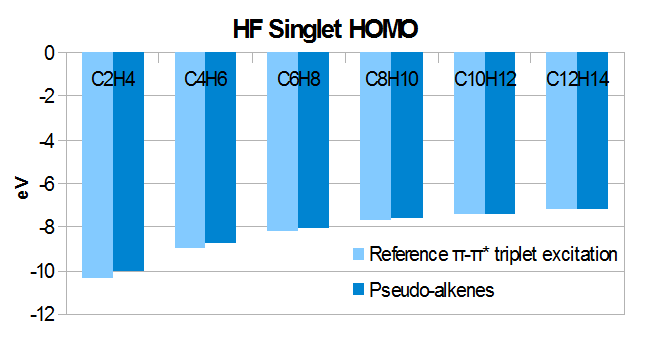
\includegraphics[width=8cm]{hf_homo}
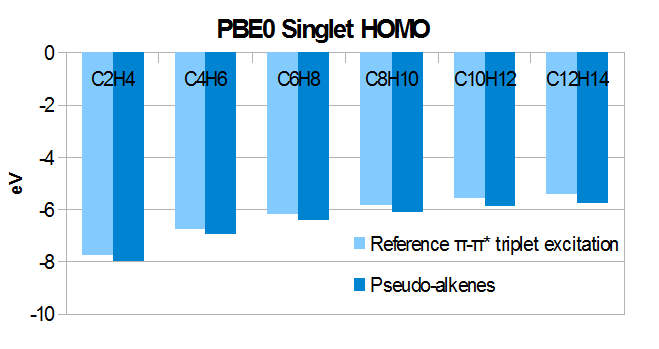
\includegraphics[width=8cm]{pbe0_homo}
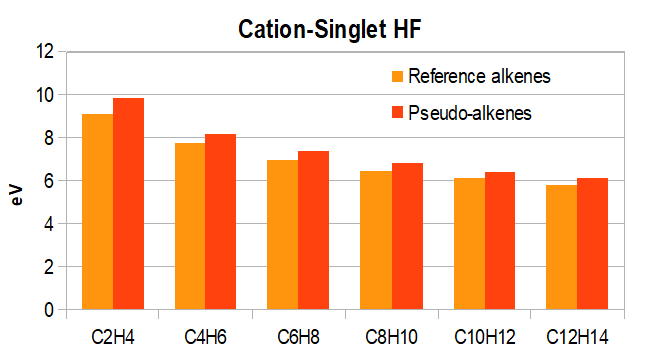
\includegraphics[width=8cm]{hf_ionisation}
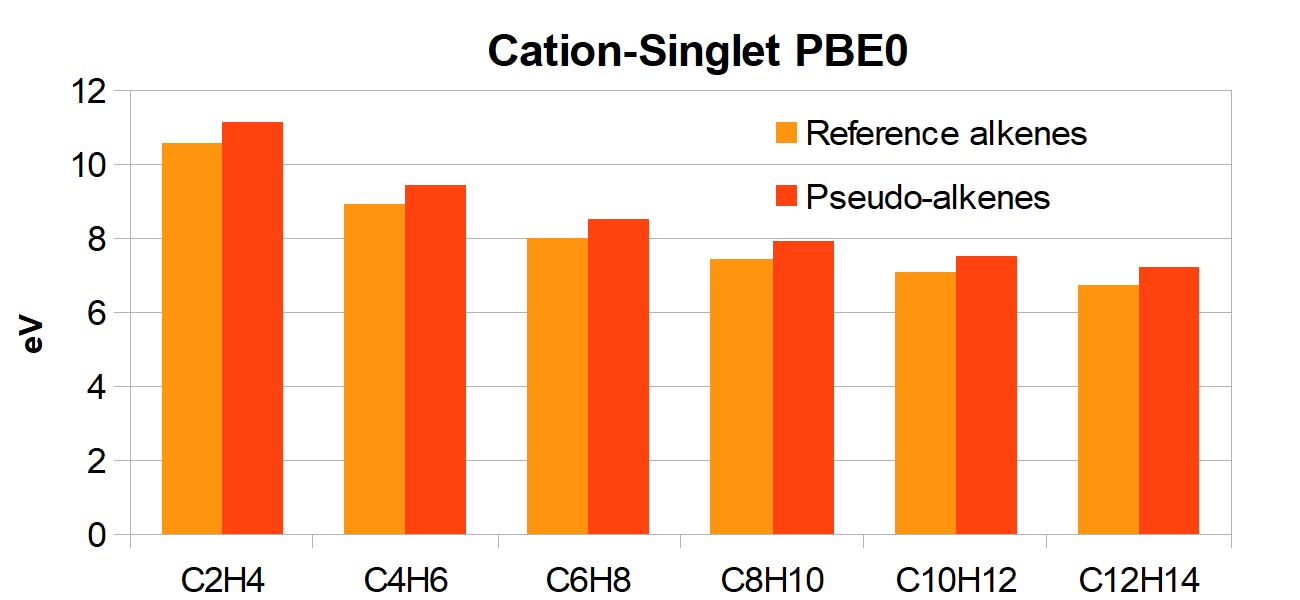
\includegraphics[width=8cm]{pbe0_ionisation}
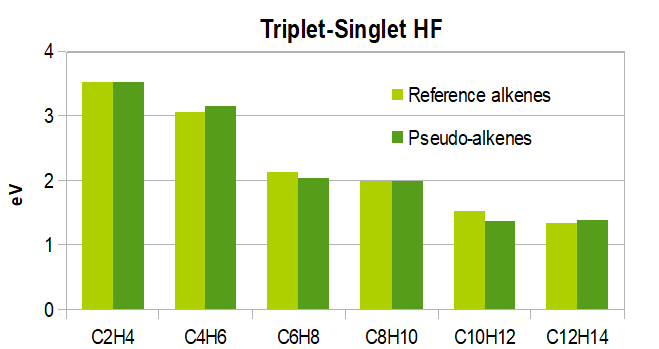
\includegraphics[width=8cm]{hf_excitation}
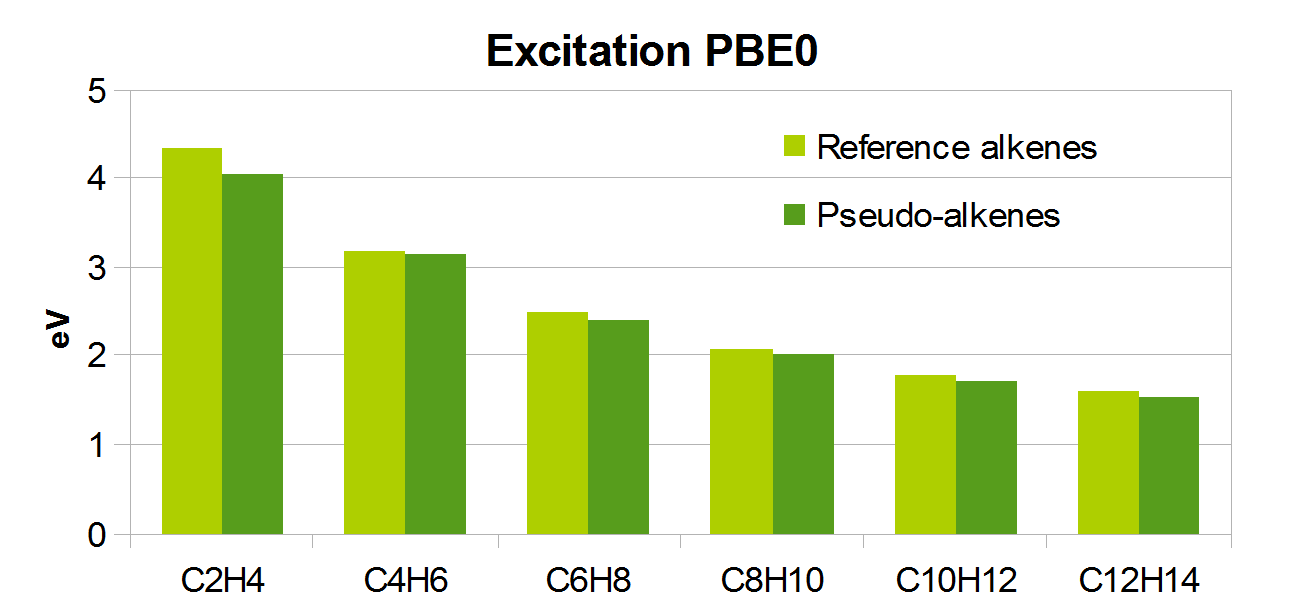
\includegraphics[width=8cm]{pbe0_excitation}
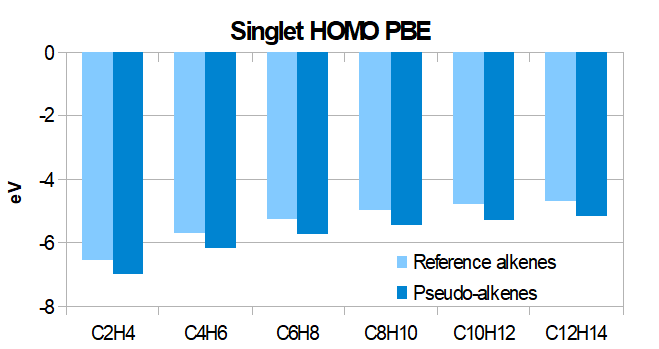
\includegraphics[width=8cm]{pbe_homo}
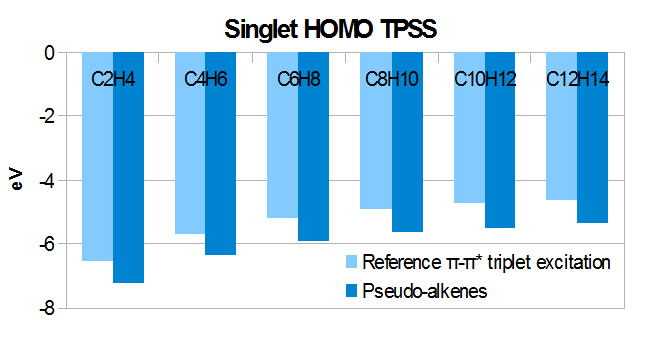
\includegraphics[width=8cm]{tpss_homo}
\end{figure}
\begin{figure}[h]
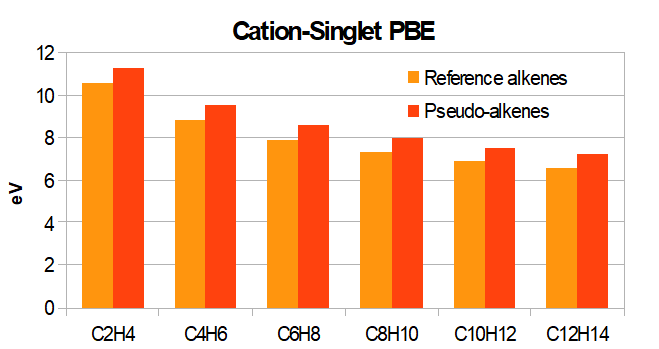
\includegraphics[width=8cm]{pbe_ionisation}
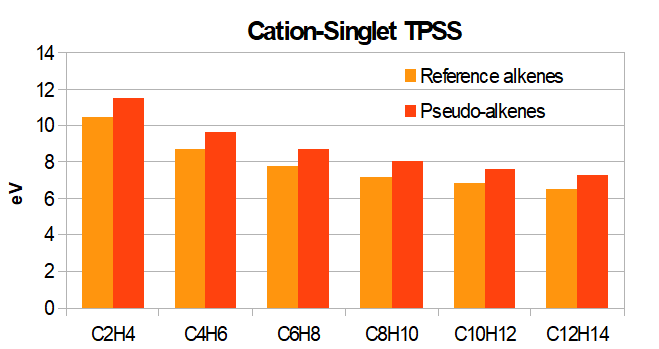
\includegraphics[width=8cm]{tpss_ionisation}
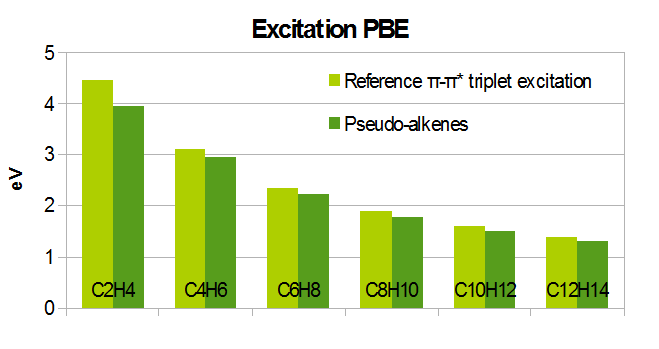
\includegraphics[width=8cm]{pbe_excitation}
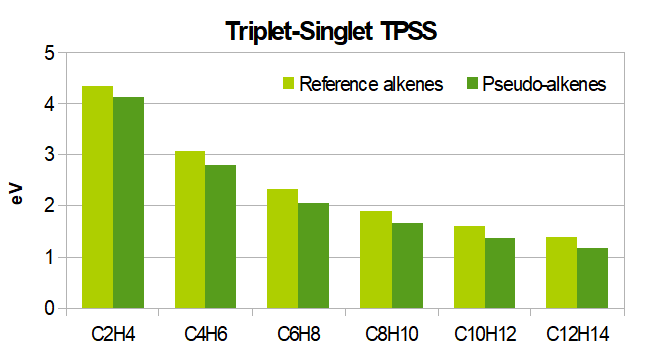
\includegraphics[width=8cm]{tpss_excitation}
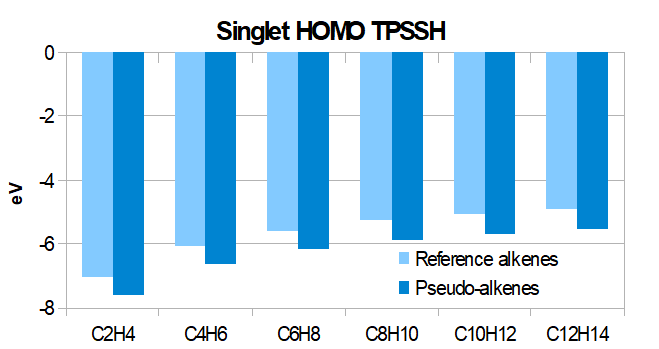
\includegraphics[width=8cm]{tpssh_homo}
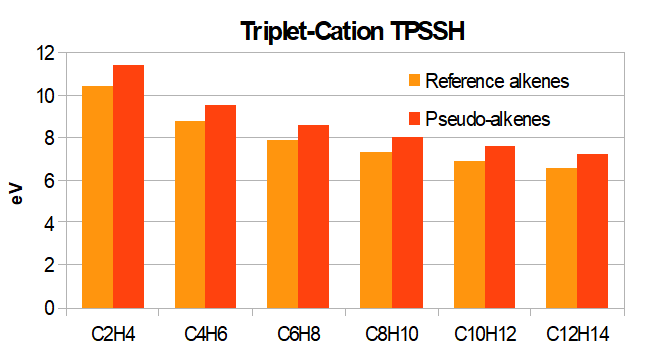
\includegraphics[width=8cm]{tpssh_ionisation}
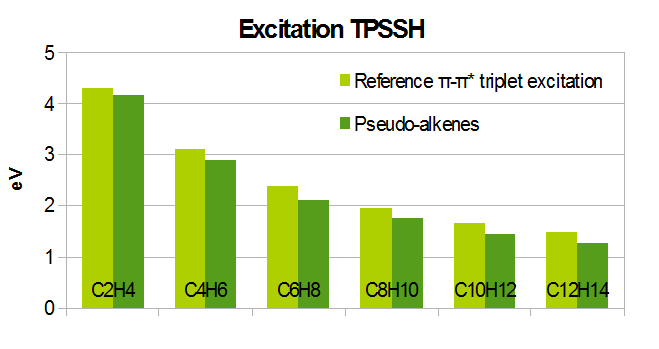
\includegraphics[width=8cm]{tpssh_excitation}
\caption{Comparison on reference and pseudo-system energies across a range of chain alkenes and computational methods.}
\label{fig:alkenes_hf_dft}
\end{figure}
\begin{figure}[h]
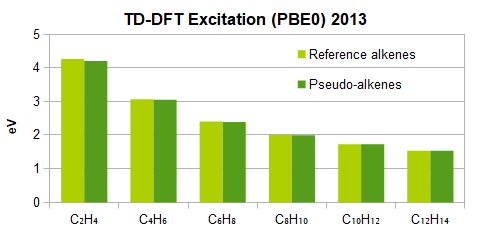
\includegraphics[width=8cm]{tddft_excitation_cd}
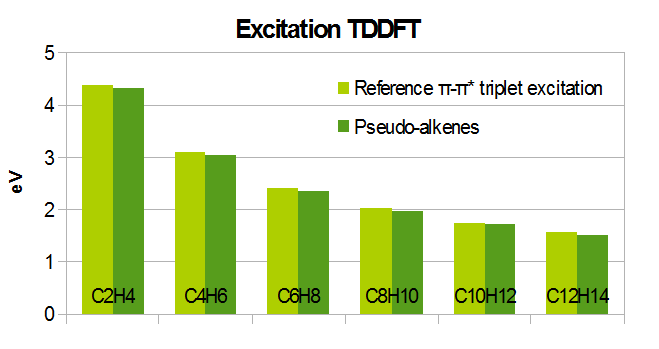
\includegraphics[width=8cm]{tddft_excitation}
\caption{Comparison of pseudo-alkenes with previous\cite{drujon_pseudopotentials_2013} and current potentials using TD-DFT excitation energies.}
\label{fig:alkenes_tddft}
\end{figure}

\begin{table}[h]
\caption{\%-errors across calculation types for short chain alkenes  (C\(_{2}\)-C\(_{12}\))}
\begin{tabular}{c c c c c c c}
\hline
Calculation Type & HF & PBE0 & PBE & TPSS & TPSSh & TD-DFT \\
\hline\hline
Mean \(\pi - \pi*\) Excitation error (\%) & 4.1 & 3.6 & 7.5 & 13.3 & 11.4 & 2.6 \\
Mean Ionisation error (\%) & 5.3 & 6.0 & 8.1 & 10.1 & 9.0 & - \\
Mean Singlet HOMO error (\%) & 1.3 & 4.0 & 8.5 & 12.0 & 9.7 & - \\
\hline
\end{tabular}
\label{table:alkene_errors}
\end{table}

\subsection{Large Systems}

The potentials derived above are also tested on larger systems. Figure \ref{fig:rings_graphs} shows the excitation, ionisation and HOMO energies for several ring systems. As with the short chain alkenes, the general trend of the results is well-replicated by the pseudo-systems, and the percentage errors, displayed in Table \ref{table:ring_system_errors}, are similar.

\begin{table}[h]
\caption{\%-errors across calculation types for ring-systems}
\begin{tabular}{c c c c c c c}
\hline
Calculation Type & HF & PBE0 & PBE & TPSS & TPSSH \\
\hline\hline
Mean \(\pi - \pi*\) Excitation error (\%) & 3.3 & 1.9 & 1.7 & 6.8 & 6.7 \\
Mean Ionisation error (\%) & 7.4 & 10.0 & 12.5 & 14.4 & 13.0 \\
Mean Singlet HOMO error (\%) & 3.4  & 9.3  & 13.4 & 17.1 & 14.7 \\
\hline
\end{tabular}
\label{table:ring_system_errors}
\end{table}

\begin{table}[h]
\caption{\%-errors across calculation types for long chain alkenes (C\(_{20}\)-C\(_{100}\))}
\begin{tabular}{c c c c c c c}
\hline\hline
Calculation Type & HF & PBE0 & PBE & TPSS & TPSSH \\
\hline
Mean \(\pi - \pi*\) Excitation error (\%) & \(\leq\)  &\(\leq\) & \(\leq\)  & \(\leq\)  & \(\leq\)  \\
Mean Ionisation error (\%) & \(\leq\)  & \(\leq\)  & \(\leq\)  & \(\leq\)  & \(\leq\)  \\
Mean Singlet HOMO error (\%) & \(\leq\)  & \(\leq\)  & \(\leq\)  & \(\leq\)  & \(\leq\) \\
\hline
\end{tabular}
\label{table:long_alkene_errors}
\end{table}

Table \ref{table:long_alkene_errors} gives the same energy details for longer chain alkenes. The pattern of decreasing ionisation and excitation energies with increasing HOMO energy is still followed, with the absolute error remaining consistent. However, with chains of this length the excitation energies begin to become smaller than the systematic error between the pseudo-system and reference system results. It is apparent that the pseudo-potentials will need to be more accurate if they are to be useful for studying these molecules.

\begin{figure}[h]
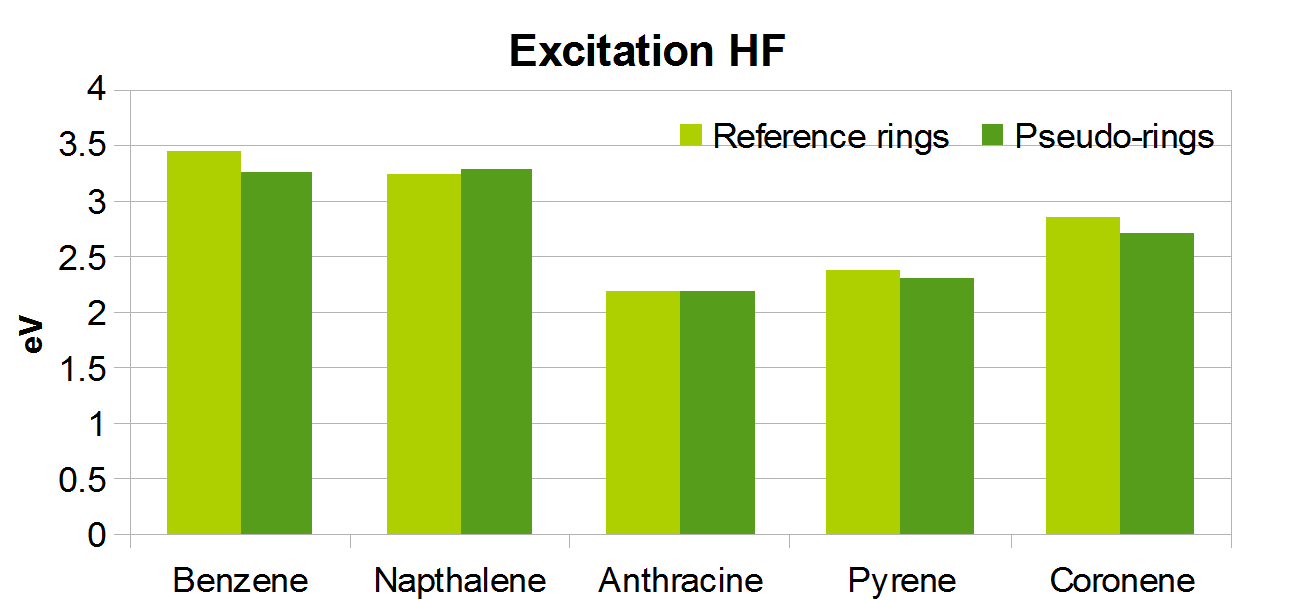
\includegraphics[width=8cm]{ring_hf_excitation}
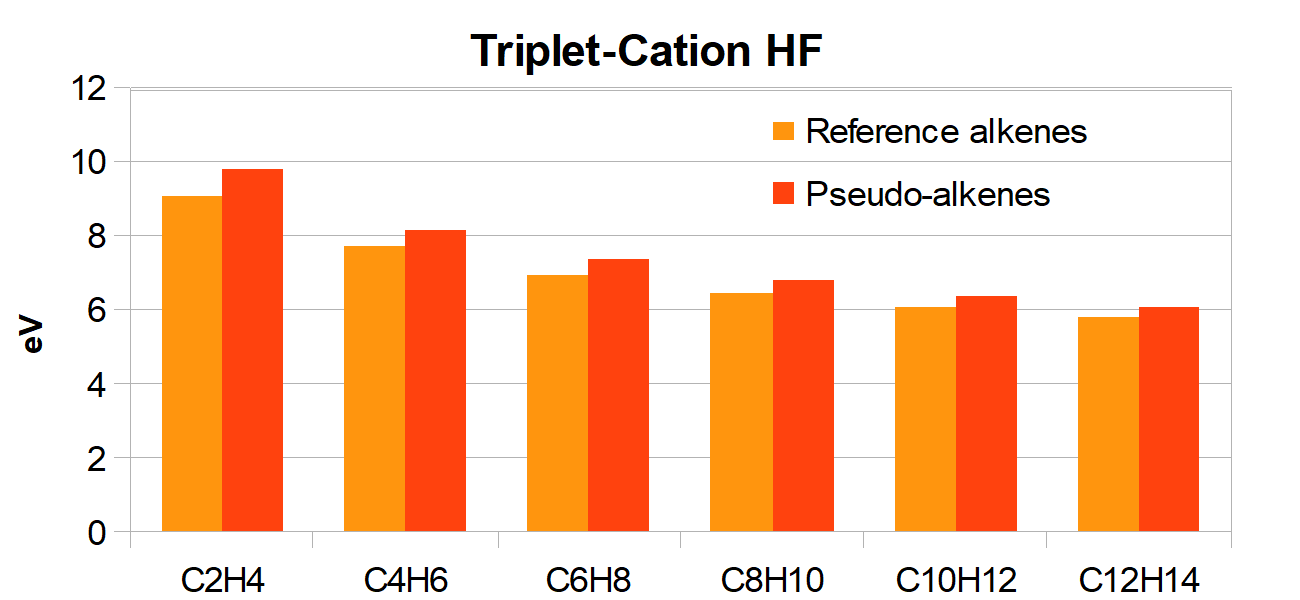
\includegraphics[width=8cm]{ring_hf_ionisation}
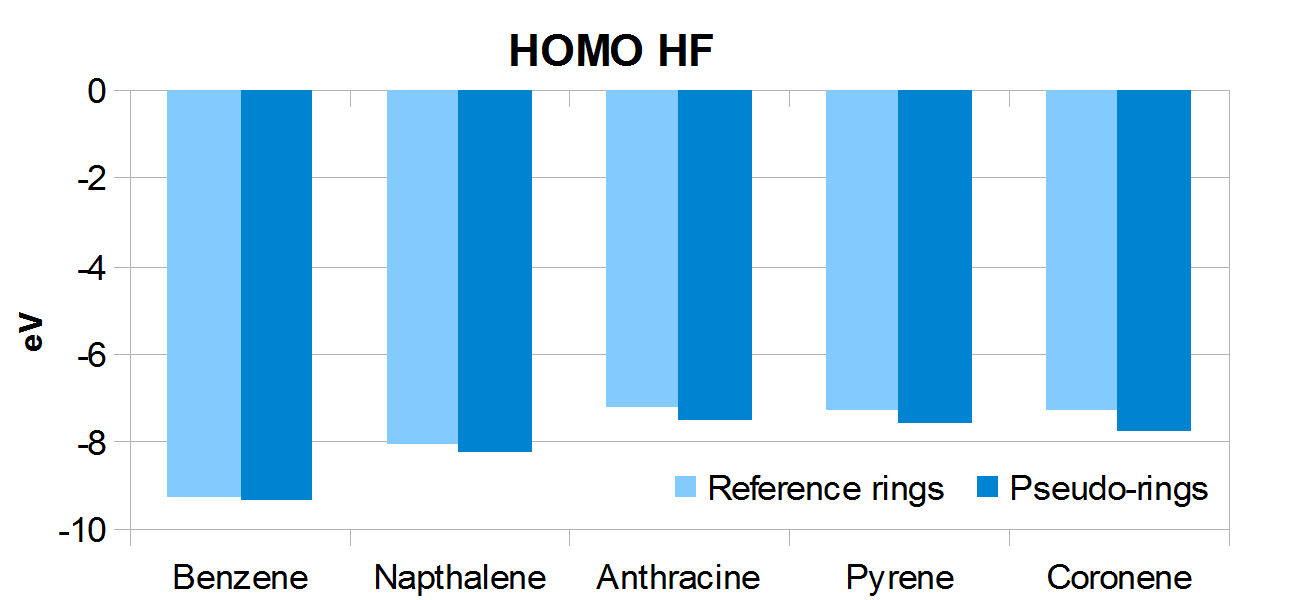
\includegraphics[width=8cm]{ring_hf_homo}
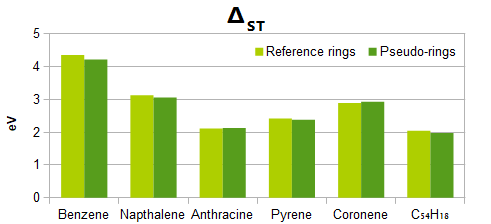
\includegraphics[width=8cm]{ring_pbe0_excitation}
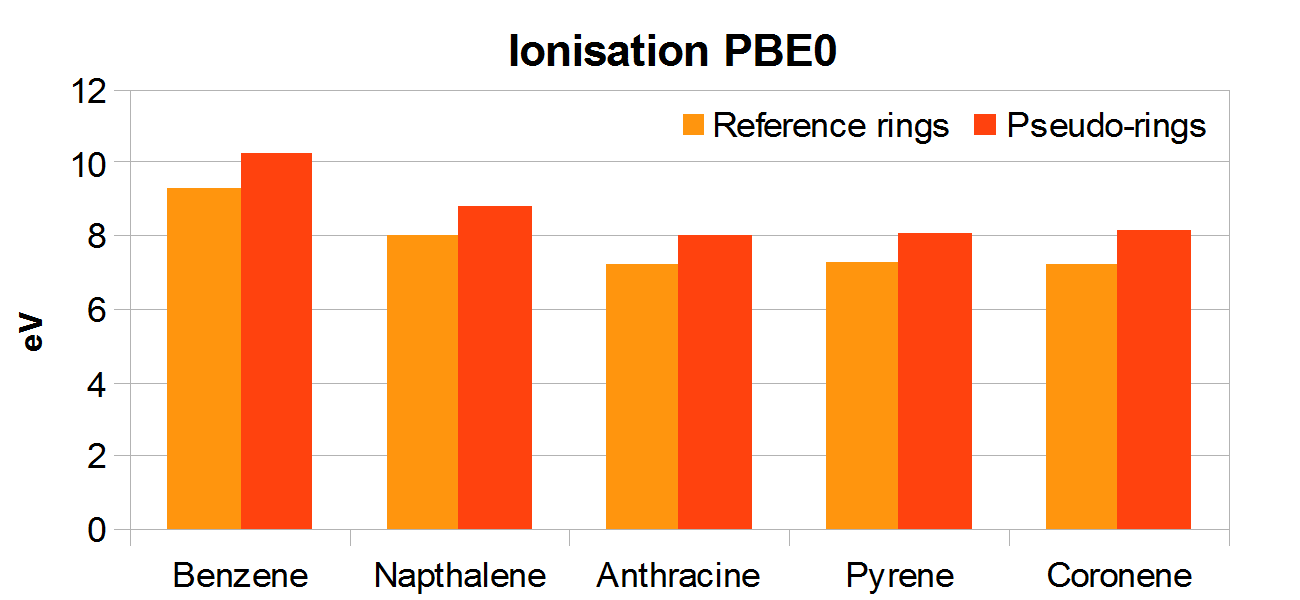
\includegraphics[width=8cm]{ring_pbe0_ionisation}
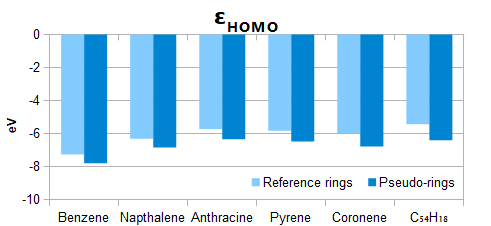
\includegraphics[width=8cm]{ring_pbe0_homo}
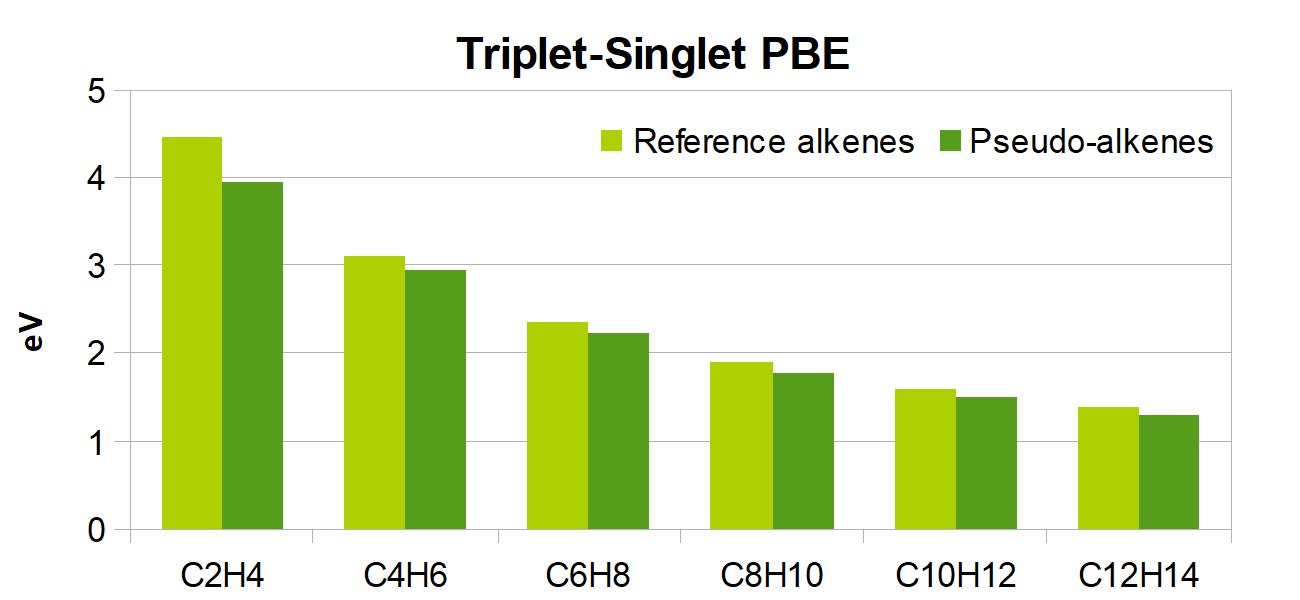
\includegraphics[width=8cm]{ring_pbe_excitation}
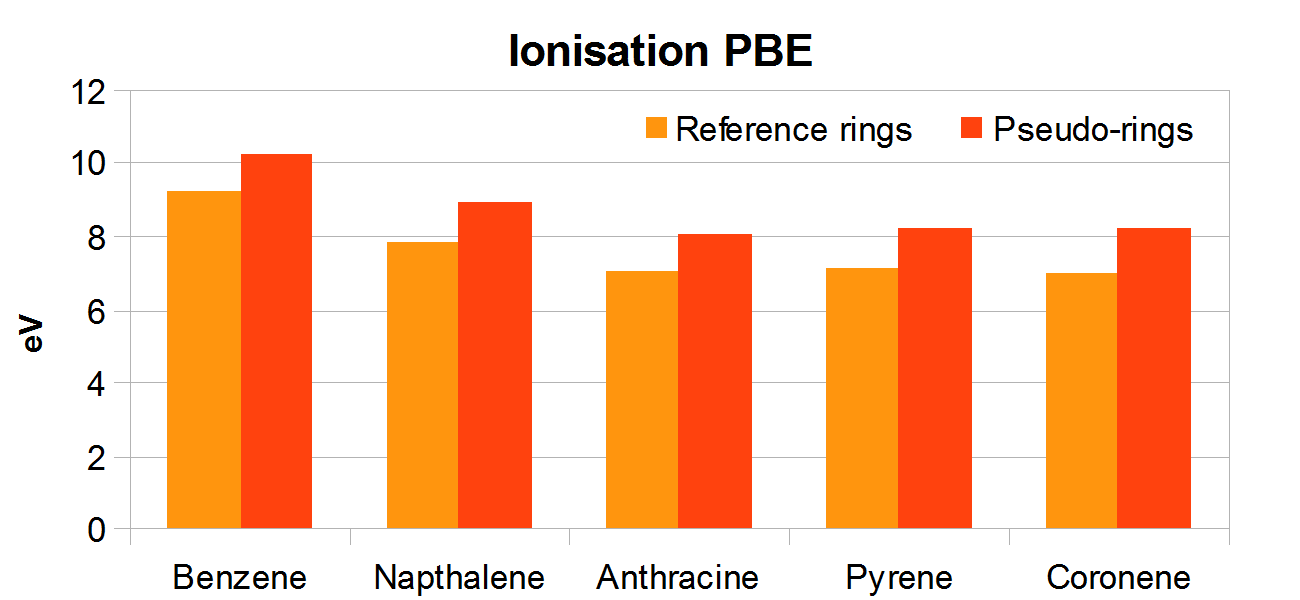
\includegraphics[width=8cm]{ring_pbe_ionisation}
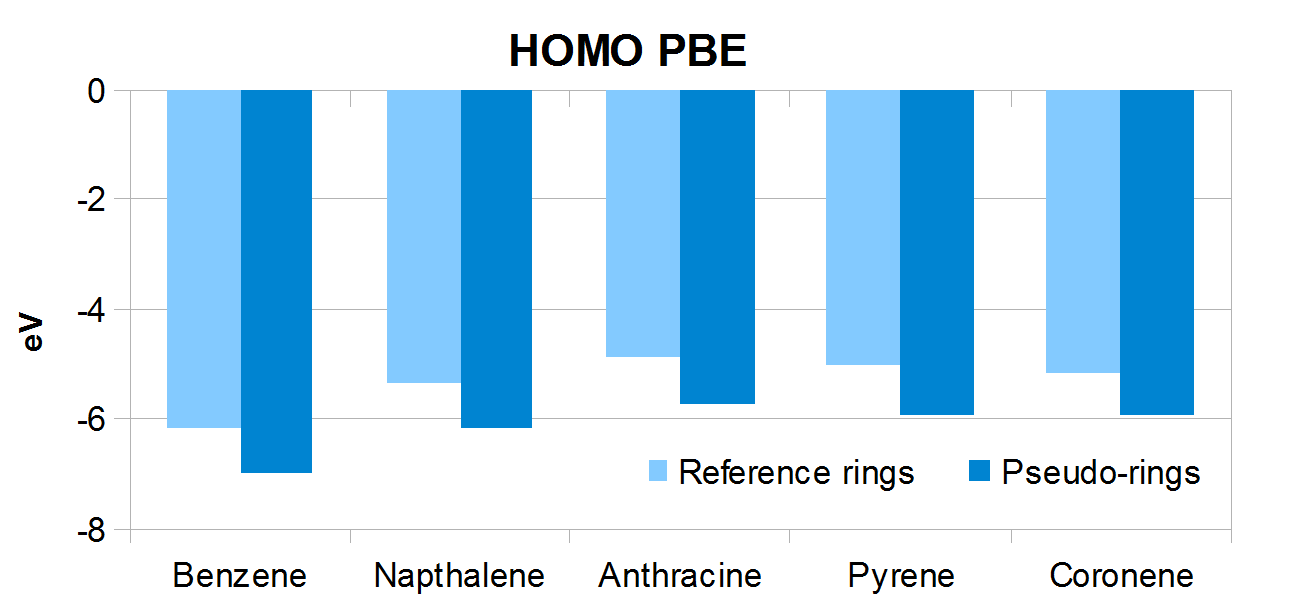
\includegraphics[width=8cm]{ring_pbe_homo}
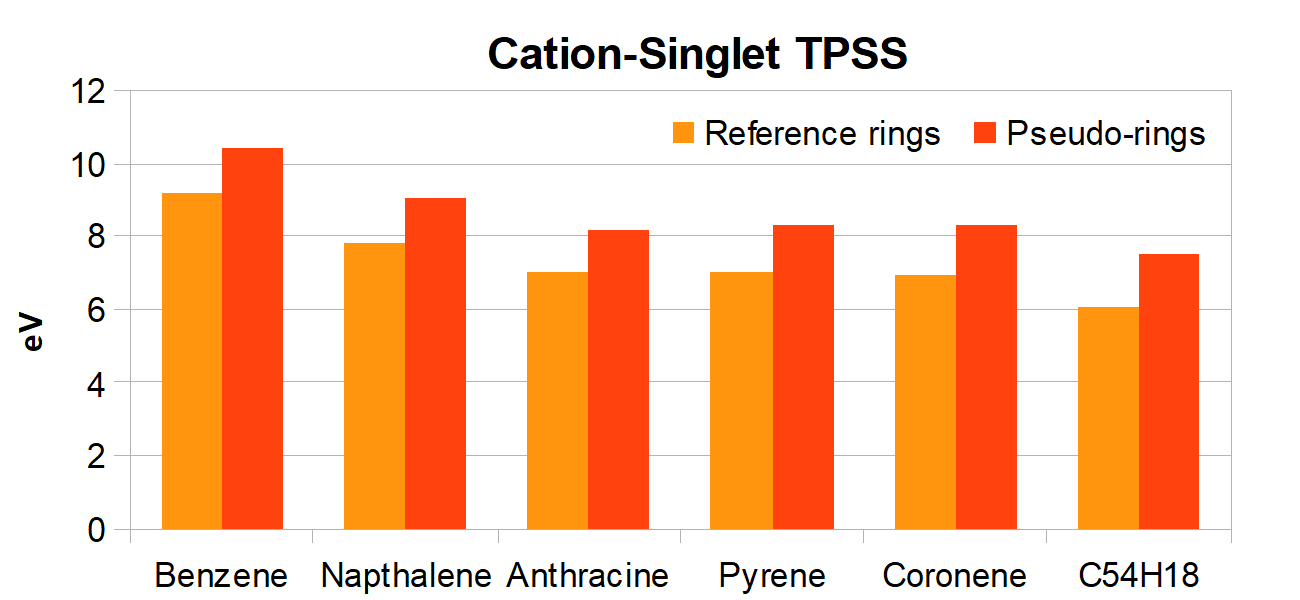
\includegraphics[width=8cm]{ring_tpss_ionisation}
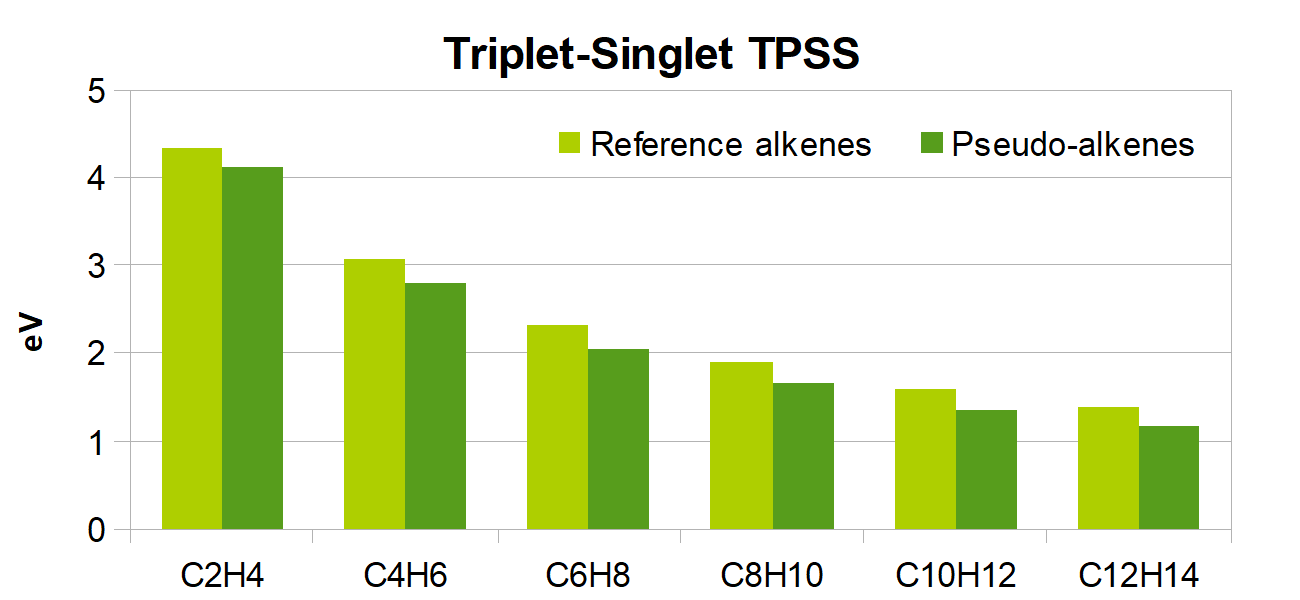
\includegraphics[width=8cm]{ring_tpss_excitation}
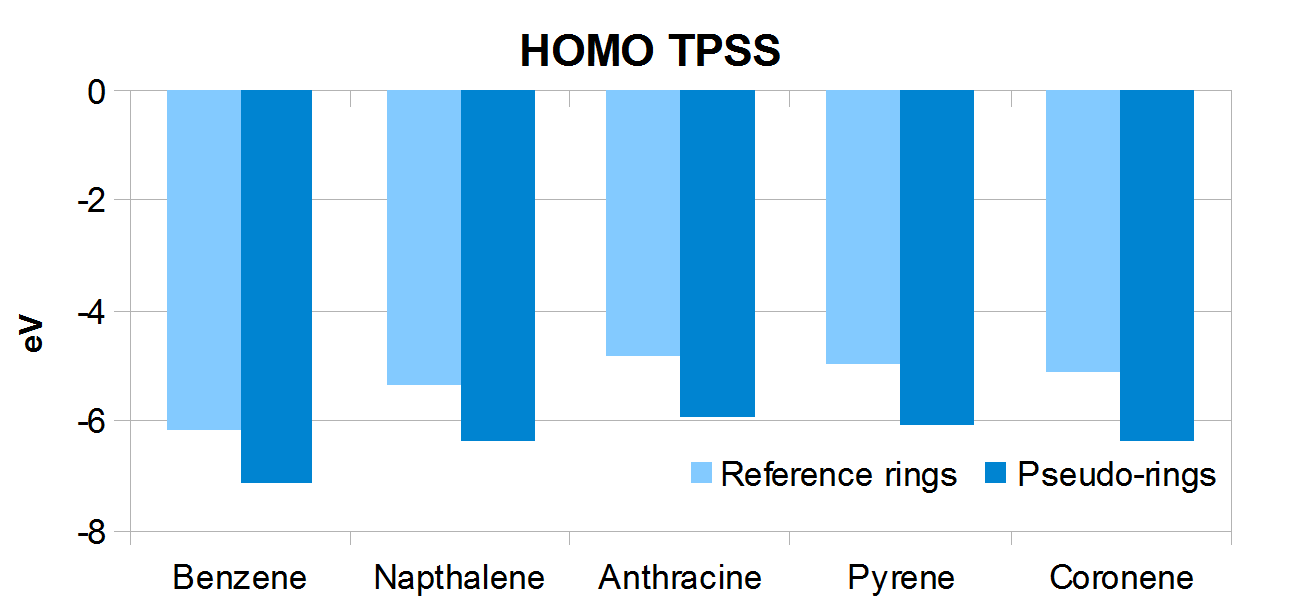
\includegraphics[width=8cm]{ring_tpss_homo}
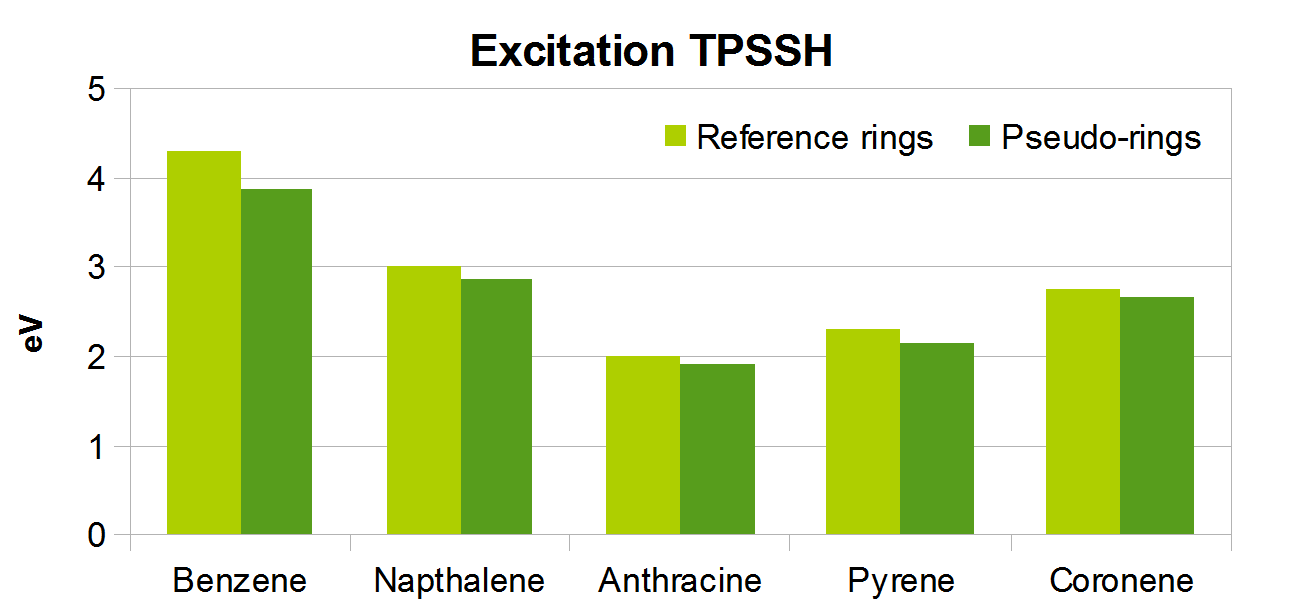
\includegraphics[width=8cm]{ring_tpssh_excitation}
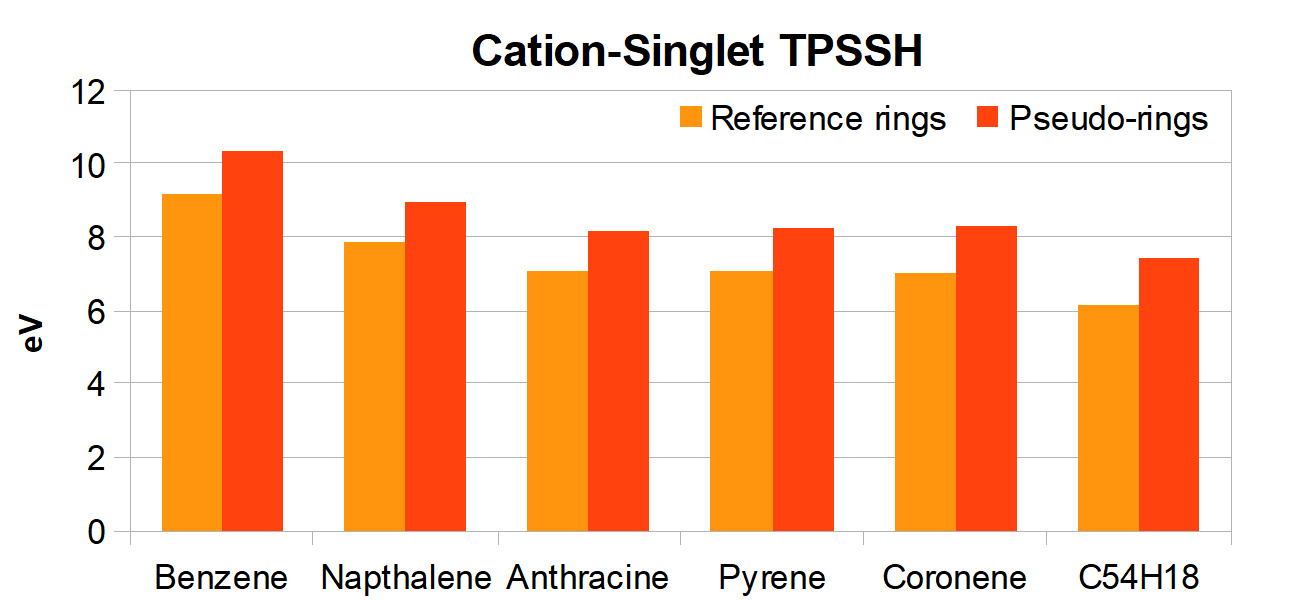
\includegraphics[width=8cm]{ring_tpssh_ionisation}
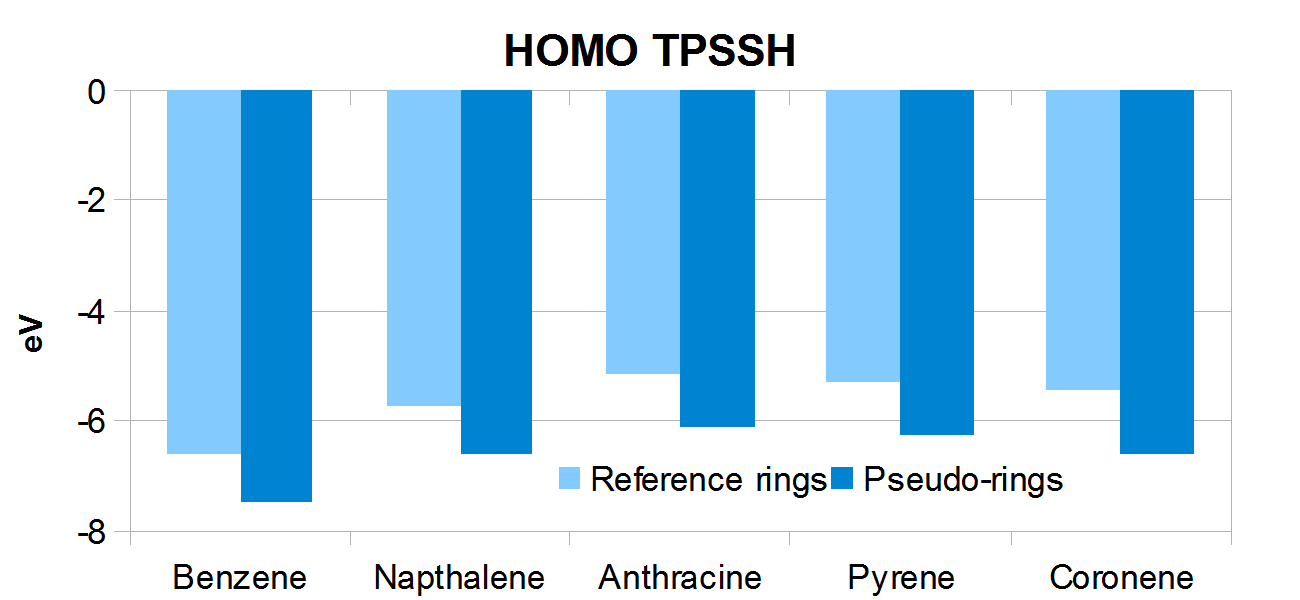
\includegraphics[width=8cm]{ring_tpssh_homo}
\caption{Comparison on reference and pseudo-system energies across a range of ring molecules and computational methods.}
\label{fig:rings_graphs}
\end{figure}

\subsection{Optimisation}

In earlier calculations with only \(s\)-potentials, optimisation was performed by choosing a range of exponent values and attempting to optimise the coefficient at each to produce the HOMO reference energy. Once the \(p_{z}\) potential was added, the \(s\)-potentials were optimised afterward. 

Once we started to look at excitation and ionisation energies however, optimisation became more complicated. Optimisations were at first performed of the s and p-potentials to reach the HOMO energy of ethene as before. With the different potential variables available, we produced a range of optimised potential sets. The best set of these potentials was then chosen and the values altered by hand in order to match as closely as possible three separate reference values: the singlet HOMO energy, the singlet-triplet \(\pi-\pi*\) excitation energy, and the first ionisation energy. All optimisations used the Brent method in SciPy's optimisation library, with a tolerance of \(1.48*10^{-08}\) \cite{scipy}, and used standard Hartree-Fock calculations.

%%%%%%%%%%%%%%%%%%%%%%%%%%%%%%%%%%%%%%%%%%%%%%%%%%%%%%%%%%%%%%%%%%%%%
%% The "Acknowledgement" section can be given in all manuscript
%% classes.  This should be given within the "acknowledgement"
%% environment, which will make the correct section or running title.
%%%%%%%%%%%%%%%%%%%%%%%%%%%%%%%%%%%%%%%%%%%%%%%%%%%%%%%%%%%%%%%%%%%%%
\begin{acknowledgement}

The authors thank \ldots

\end{acknowledgement}

- radical dot in CH3 DONE

- C - H distiance in optimised radical (+optimisation details)

- line 73 "As we want to avoid to modifiy the quantum chemistry software itself, the pseudopotentials have a semilocal form and we choose a value of n=1 to preserve the 1/r behaviour as huzinanaga's work". DONE

- We are not aiming to exactly reproduce reference values. We aim to give physically relevant effects to the potentials. To go further than huckel or tight-binding models, allowing the study of more than first-neighbour effects. our systems is completely delocalised. (We aren't actually making use of the physical assumptions of the mdoel to probe new systems here, one of the posited potential uses of it). And computational time.

- line 74 make explicit that we aren't aiming to duplicate a bielctronic interaction with a mono-electric one. DONE

- line 75: The PPs are monoelectronic operators, thus they shall not be able to reproduce fully bielectronic interactions. Knowing this, we adjust the parameters of the s potentials for the pseudosystem to have a wavefunction in which properties are as close as possible to those of the reference system, such as spatial extent, energy and excitation energies. DONE

- line 76-80. emphasise lack of H atoms. Colon line 76. DONE

- line 83 Here / in this article. Potatoes. DONE

- line 87 Slater reference DONE

- line 88 details of z = 2.4 calc?

- lie 91 Zeff is Z. Define it. DONE

- you might not need line 92. these equations are not used again. comment out for now DONE

- line 95. state exactly what the mean r is from or for. "our" calculation? DONE

- line 101-104: Don't need sentence beginning "However, ..". Remove word "matrix". DONE

- line 101-104: Query reference

- line 101-104: Rather than sentence beginning however: "Even if we shall use the semi-local pseudopotential definition for the calculations, for a 
quick evaluation of overlap effects between the basis set and the pseudopotential, we assume a non-local psedopotential definition. We define: S = [Equation], ..." DONE

- Section 2.3.1 refers to calculationss yet to come, and can be moved to after section 3. DONE

- line 120: delete the reasons, nobody cares. DONE

- sections 3.1 and 3.2 emphasise in titles the use of s and p potentials DONE

- table 1: some detail of geometry optimisation (and functional / basis set)

- table 4 and 5 can be unified DONE

- Merge reference values in table 1 into the relevant pseudotables

- line 145: ONLY s potentials DONE

- a.u. for all distances DONE

- more detail (d) in table 2 title

- section 3.3. header can move downa  bit to after ethene optimisation DONE

- emphasise addition of p potential DONE

- line 158 "along the z axis" no. DONE

- line 160 proceeeeeeeeeeeeeeeeeeeeeeeeeeedure. DONE

- table 4 is not needed. DONE

- table 5: d = 0.5 DONE

- line 186 c + D

- tables 6 and 7 could be merged, table 6 needs ref values, or table 7 could be before 6 DONE

- Need final coeffs and exps DONE

- maybe all the potential sets used could be consolidated into one table, easy to refer to?

- some pictures of pseudomolecules

%%%%%%%%%%%%%%%%%%%%%%%%%%%%%%%%%%%%%%%%%%%%%%%%%%%%%%%%%%%%%%%%%%%%%
%% The same is true for Supporting Information, which should use the
%% suppinfo environment.
%%%%%%%%%%%%%%%%%%%%%%%%%%%%%%%%%%%%%%%%%%%%%%%%%%%%%%%%%%%%%%%%%%%%%
\begin{suppinfo}

A listing of the contents of each file supplied as Supporting Information
should be included. For instructions on what should be included in the
Supporting Information as well as how to prepare this material for
publications, refer to the journal's Instructions for Authors.

The following files are available free of charge.
\begin{itemize}
  \item Filename: brief description
  \item Filename: brief description
\end{itemize}

\end{suppinfo}

%%%%%%%%%%%%%%%%%%%%%%%%%%%%%%%%%%%%%%%%%%%%%%%%%%%%%%%%%%%%%%%%%%%%%
%% The appropriate \bibliography command should be placed here.
%% Notice that the class file automatically sets \bibliographystyle
%% and also names the section correctly.
%%%%%%%%%%%%%%%%%%%%%%%%%%%%%%%%%%%%%%%%%%%%%%%%%%%%%%%%%%%%%%%%%%%%%
\bibliography{biblio_pseudo_alex}

\end{document}
